\chapter{IDF Editor -- Brief Introduction}\label{idf-editor-brief-introduction}

EnergyPlus has several options for the user to create input files. For the purposes of this document, we will describe briefly the workings of the IDF Editor that is supplied with the EnergyPlus Installation.~ The IDF Editor is a simple, ``intelligent'' editor that reads the EnergyPlus Data Dictionary (IDD) and allows creation/revision of EnergyPlus Input Files (IDF). It can be run from a shortcut in the main EnergyPlus directory (created as part of the install) or directly from EP-Launch.

Full details of the IDF Editor can be found in the Auxiliary Programs document.~ IDD Conventions (to be able to read the IDD) are found in the Input Output Reference document. EnergyPlus standard units are described in several places, including later in this document.

IDF Editor is an optional component of the EnergyPlus installation. For users who want a simple way of creating or editing EnergyPlus input data files (IDF), IDF Editor provides this service.~ The IDF Editor does not check inputs for validity, although some numeric fields are highlighted if out of range and some text fields are highlighted if they contain an invalid reference. For instructions and rules that must be followed when creating an IDF file the user should refer to the \href{../../EnergyPlusFromStarTeam/EnergyPlusFromStarTeam/Documentation/sources/InputOutputReference.pdf}{\emph{Input/Output Reference}} document.

\begin{figure}[hbtp] % fig 21
\centering
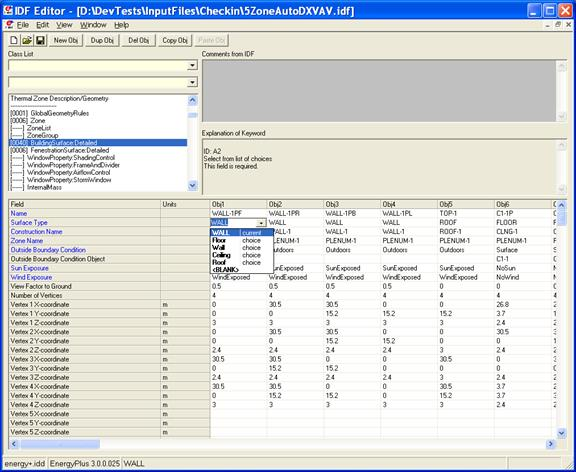
\includegraphics[width=0.9\textwidth, height=0.9\textheight, keepaspectratio=true]{media/image021.jpg}
\caption{IDF Editor Screen. \protect \label{fig:idf-editor-screen.}}
\end{figure}

\subsection{Start IDF Editor}\label{start-idf-editor}

IDF Editor should be located in the EnergyPlus\textbackslash{}PreProcessor\textbackslash{}IDFEditor directory where you installed EnergyPlus. By double clicking on the IDF Editor icon you will get a screen similar to the one shown above. IDF Editor works in conjunction with the current EnergyPlus Input Data Directory (IDD) file that resides in the directory where EnergyPlus is installed. Another way to start the IDF Editor is from EP-Launch. Multiple IDF files can be opened at once.

\subsection{Creating or Selecting an Input Data File}\label{creating-or-selecting-an-input-data-file}

Creating a new input data file or selecting an existing input data file can be accomplished either through use of the File menu on the menu bar at the top of the screen or through use of the New File icon button or Open File icon button on the tool bar.

\subsection{Class List}\label{class-list}

The class list shows how the items for the IDF are grouped.~ This class list follows the Data Dictionary (IDD) description. Select a class from the list by clicking on and highlighting the class. The field to the left of the selected class in the `Class List' will either contain {[}------{]} to indicate that this class has no objects in the IDF file or it will contain a number like {[}0003{]} to indicate the number of times the object currently appears in the IDF file. For example, for the BuildingSurface:Detailed class selected in the screen above under the Thermal Zone Description/Geometry group, there are 40 objects in the IDF file. The details for these 40 objects or any new object that is defined are displayed in columns within the grid. Each object is made up of fields and can be used to further define the object. Any units attached to each field are shown in the second column. You may need to scroll down the `field' list or maximize the application to see all of the fields. Likewise, you may need to scroll to the right of the main grid to see other objects.

Options under the view menu can change how you use the Class List. To display only classes that contain objects select the ``show classes with objects only'' option on the ``View'' menu. You can also toggle this feature on and off with CTRL+L. If the file is empty and has no objects, this toggle does not impact the display.

The ``Show Quick Select Dropdowns'' view menu option adds two new input fields to the main screen. The input fields can be used to go quickly to different classes in the main list of classes. By typing in the top input field, the group that start with those letters are displayed. After selecting one and pressing the tab button, classes in that group are shown and by typing the first few letters, you can easily select a specific class. Pressing tab again displays that class and it objects. This method allow for quick selection of classes if you remember the group name and class name.

\subsection{Changing Values}\label{changing-values}

By clicking and highlighting a value within an object, several things happen:

1)~~~Any user comments from the IDF file will be displayed in the `Comments from IDF' portion of the screen

2)~~~Any notes contained in the IDD for this input field will be displayed in the `Explanation of Keyword' portion of the screen

3)~~~The value can be edited. Depending on the field, a drop down list may display the default value, maximum and minimum, or other keywords that can be used with the field.

4)~~~Numeric fields that can be autosized will include ``autosize'' as a selection in the drop down list.

5)~~~Some numeric fields have a maximum and/or minimum value specified in the IDD. If the value entered is outside this range, the cell will be highlighted in pale orange.

6)~~~For values that are names of nodes, a new dialog box titled ``Edit or Select Node Name'' can be shown when the small button is pressed that is on the right side in each node name cell.

\subsection{Working with Objects}\label{working-with-objects}

To delete an object, first click on any value for the object and then click on the ``Del Obj'' button. To add a new object, click on the ``New Obj'' button and a new object column with fields set to blanks, zeros, or default values will be added to the far right of the grid. The ``Dup Obj'' button is similar to ``New Obj'', but copies the values of the fields of the currently selected object. Copying and pasting an object or groups of objects is also possible using the ``Copy Obj'' and ``Paste Obj'' buttons.~ These allow objects to be copied between files are also good for copying from files in the DataSets subdirectory. (Also see the Edit menu to perform these functions.)

\subsection{File Menu}\label{file-menu-000}

The File menu can be used for creating or selecting input files just like the buttons on the IDF Editor screen (see the \emph{Creating or Selecting an Input File} section above). In addition, the File menu is used to save a file or exit the IDF Editor. More than one file can be opened at a time.

The ``File'', ``Save Options'' screen is shown below.

~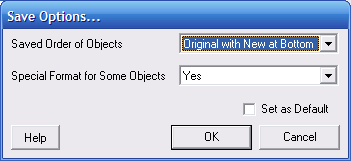
\includegraphics{media/image022.png}

Figure 22. IDF Editor Save Options Screen.

The save options allow the order of the objects in the file to be sorted by type of object or to keep the original order of the objects (for an existing file). The placement of new objects when the original order is specified can be either at the top or bottom of the file.

In addition, the Save Options also allow certain objects to be written to the file using a specific format that some users prefer. Selecting this option will format the following objects on a single line: Report, Report Meter, Report Variable, Version, Timestep in Hour, Inside Convection Algorithm, Outside Convection Algorithm, Solution Algorithm, Shadowing Calculations, Ground Reflectances, and GroundTemperatures:Deep. In addition, Schedule:Compact objects will be formatted to have two field for some lines. With this option, objects with geometric vertices are formatted to have the X, Y, and Z values on the same line. Those objects include: Surface:HeatTransfer, Surface:HeatTransfer:Sub, Surface:Shading:Detached:Fixed, Surface:Shading:Detached:Building and Surface:Shading:Attached.

The settings for the save options are kept for each file saved from the IDF Editor.

Also on the File menu is the Open DataSet menu and submenu. This allows you to open any input file that appears in the DataSet subdirectory and copy objects from them into another file. This is required because EnergyPlus does not read the DataSet files, it is up to you to include objects from them.

\subsection{Edit Menu}\label{edit-menu-000}

The Edit Menu offers options to create a new object, duplicate an object, and delete an object as well as finding and searching. The object options are the same operations as can be accomplished by using the `New Obj', `Dup Obj' and `Del Obj' buttons (see the \emph{Working with Objects} section above). In addition, the ``Next Row after Enter'' option can be toggled. When this option is on, the selection moves down one row after pressing Enter. The copy and paste object commands allow a single object to be copied within a file or between files. The pasted object appears as the last object in the class. This capability makes it easier to utilize the data in the DataSets directory. The Find Class and Search and Replace options can be used to search through the list of classes or the values of a file quickly. If renaming objects, the recommended approach is to rename the object and select the cell again and open the Search and Replace dialog. This will show other places in the file that use that object name that also may need to be changed.

\subsection{View Menu}\label{view-menu-000}

The View menu offers options for units and column widths. The Narrow/Medium/Wide Column options set the standard column width for items in the object grid. Individual columns can also be resized by dragging the column separator. The displayed value is rounded and/or expressed in scientific notation to fit within the column width.

EnergyPlus input files must always be in SI units. Selecting ``Inch-Pound'' (IP) units in the View menu displays and edits values in IP units.

1)~~~The IP unit will be displayed in the units column of the object grid. Some SI units convert to multiple IP units. For example, W becomes Btu/hr for heating and cooling capacity but remains as W for lighting and electrical equipment.

2)~~~All conversion factors used in the IDF editor are documented in a block of comments near the top of the Energy+.IDD file.

3)~~~Schedules, fluid properties and curves now support IP unit conversions. For curves, the minimum and maximum values are converted but the coefficients are not.

To display only classes that contain objects select the ``show classes with objects only'' option on the ``View'' menu. You can also toggle this feature on and off with CTRL+L. If the file is empty and has no objects, this toggle does not impact the display.

The ``Show Quick Select Dropdowns'' view menu option adds two new input fields to the main screen. The input fields can be used to go quickly to different classes in the main list of classes.

The ``Validity Check'' function has replaced and expanded upon the old~ ``Check Out-of-Range'' function. It can also be started by using CTRL-R. The ``Validity Check'' function performs three kinds of validity checks. It displays the values and locations for objects with values that are either above the maximum or below the minimum values.~ It also displays fields that contain invalid references. The ``Validity Check'' dialog also shows when an entry for a field is not one of the possible lists of choices. The Perform Validity Check When Saving File can be turned on and off and automatically performs the check whenever the file is saved.

\subsection{Help Menu}\label{help-menu-000}

The Help menu offers options to open the EnergyPlus documentation files.
